\documentclass[border=4pt]{standalone}
\usepackage{amsmath,amssymb}
\usepackage[scaled=0.92]{helvet}
\renewcommand{\familydefault}{\sfdefault}
\usepackage{tikz}
\usetikzlibrary{positioning,arrows.meta,fit,backgrounds,calc}
\definecolor{cInD}{HTML}{3B6EA8}
\definecolor{cGD}{HTML}{C76E00}
\definecolor{cTD}{HTML}{2E7D32}
\definecolor{cOD}{HTML}{7B3F99}
\definecolor{cRD}{HTML}{B23A3A}
\definecolor{cSH}{HTML}{3B6EA8}\definecolor{cQA}{HTML}{D9A400}\definecolor{cKD}{HTML}{D2691E}
\tikzset{
  box/.style={draw=#1!80!black, fill=#1!10, rounded corners=3pt, align=center, font=\small, inner sep=4pt, line width=0.6pt},
  arr/.style={-{Stealth[length=2.2mm]}, line width=0.8pt, draw=black!70},
  lbl/.style={font=\footnotesize, text=black!75, align=center},
  grp/.style={draw=#1, dashed, rounded corners=5pt, line width=0.7pt, inner sep=5pt},
  ttl/.style={font=\small\bfseries, text=#1, anchor=north},
}
\newcommand{\minigraph}[3]{%
  \begin{scope}[shift={#1}]
    \foreach \a/\n in {90/a,162/b,234/c,306/d,18/e}{\node[circle, fill=#2, inner sep=1.5pt] (#3\n) at (\a:0.38) {};}
    \draw[#2, line width=0.6pt] (#3a)--(#3c) (#3a)--(#3d) (#3b)--(#3e) (#3b)--(#3d) (#3c)--(#3e) (#3a)--(#3b) (#3d)--(#3e);
  \end{scope}}
\begin{document}
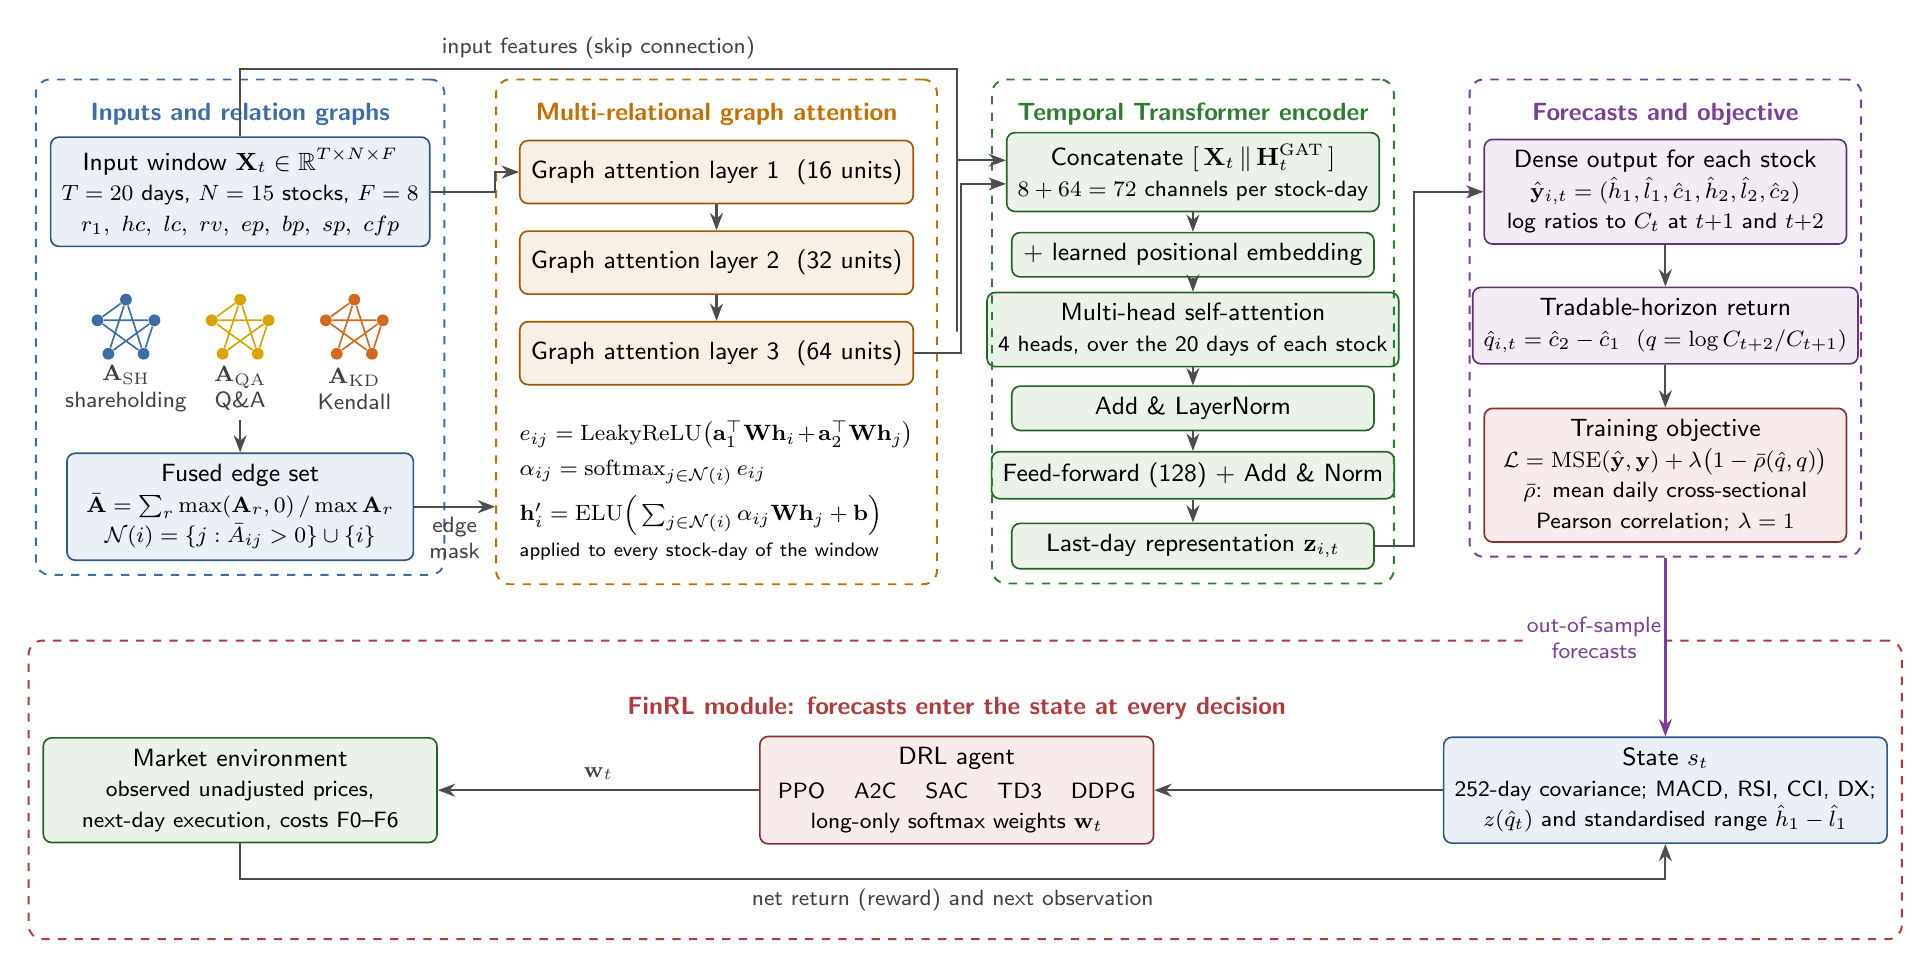
\begin{tikzpicture}
% ================= column A: inputs
\node[ttl=cInD] (tA) at (2.3,0) {Inputs and relation graphs};
\node[box=cInD, minimum width=44mm] (X) at (2.3,-1.25) {Input window $\mathbf{X}_t\in\mathbb{R}^{T\times N\times F}$\\
  {\footnotesize $T=20$ days, $N=15$ stocks, $F=8$}\\ {\footnotesize $r_1,\ hc,\ lc,\ rv,\ ep,\ bp,\ sp,\ cfp$}};
\minigraph{(0.85,-3.0)}{cSH}{s}\minigraph{(2.3,-3.0)}{cQA}{q}\minigraph{(3.75,-3.0)}{cKD}{k}
\node[lbl] at (0.85,-3.75) {$\mathbf{A}_{\mathrm{SH}}$\\ shareholding};
\node[lbl] at (2.3,-3.75) {$\mathbf{A}_{\mathrm{QA}}$\\ Q\&A};
\node[lbl] at (3.75,-3.75) {$\mathbf{A}_{\mathrm{KD}}$\\ Kendall};
\node[box=cInD, minimum width=44mm] (Abar) at (2.3,-5.25) {Fused edge set\\ {\footnotesize $\bar{\mathbf{A}}=\sum_{r}\max(\mathbf{A}_r,0)\,/\max\mathbf{A}_r$}\\ {\footnotesize $\mathcal{N}(i)=\{j:\bar A_{ij}>0\}\cup\{i\}$}};
\draw[arr] (2.3,-4.15) -- (Abar.north);
\node[grp=cInD, fit=(tA)(X)(Abar)] (gA) {};
% ================= column B: MGAT
\node[ttl=cGD] (tB) at (8.35,0) {Multi-relational graph attention};
\node[box=cGD, minimum width=46mm, minimum height=8mm] (g1) at (8.35,-1.0) {Graph attention layer 1 \ (16 units)};
\node[box=cGD, minimum width=46mm, minimum height=8mm] (g2) at (8.35,-2.15) {Graph attention layer 2 \ (32 units)};
\node[box=cGD, minimum width=46mm, minimum height=8mm] (g3) at (8.35,-3.3) {Graph attention layer 3 \ (64 units)};
\draw[arr] (g1)--(g2); \draw[arr] (g2)--(g3);
\node[font=\footnotesize, align=left, text width=50mm] (geq) at (8.35,-5.05) {%
$e_{ij}=\mathrm{LeakyReLU}\big(\mathbf{a}_1^{\top}\mathbf{W}\mathbf{h}_i+\mathbf{a}_2^{\top}\mathbf{W}\mathbf{h}_j\big)$\\[3pt]
$\alpha_{ij}=\mathrm{softmax}_{j\in\mathcal{N}(i)}\,e_{ij}$\\[3pt]
$\mathbf{h}'_i=\mathrm{ELU}\Big(\sum_{j\in\mathcal{N}(i)}\alpha_{ij}\mathbf{W}\mathbf{h}_j+\mathbf{b}\Big)$\\[2pt]
{\scriptsize applied to every stock-day of the window}};
\node[grp=cGD, fit=(tB)(g1)(geq)] (gB) {};
\draw[arr] (X.east) -- (X.east -| gB.west) |- (g1.west);
\draw[arr] (Abar.east) -- node[lbl, below]{edge\\ mask} (Abar.east -| gB.west);
% ================= column C: Transformer
\node[ttl=cTD] (tC) at (14.4,0) {Temporal Transformer encoder};
\node[box=cTD, minimum width=46mm] (cat) at (14.4,-1.0) {Concatenate $[\,\mathbf{X}_t\,\|\,\mathbf{H}^{\mathrm{GAT}}_t\,]$\\ {\footnotesize $8+64=72$ channels per stock-day}};
\node[box=cTD, minimum width=46mm] (pos) at (14.4,-2.05) {+ learned positional embedding};
\node[box=cTD, minimum width=46mm] (mha) at (14.4,-3.0) {Multi-head self-attention\\ {\footnotesize 4 heads, over the 20 days of each stock}};
\node[box=cTD, minimum width=46mm] (an1) at (14.4,-4.0) {Add \& LayerNorm};
\node[box=cTD, minimum width=46mm] (ffn) at (14.4,-4.85) {Feed-forward (128) + Add \& Norm};
\node[box=cTD, minimum width=46mm] (last) at (14.4,-5.75) {Last-day representation $\mathbf{z}_{i,t}$};
\foreach \a/\b in {cat/pos,pos/mha,mha/an1,an1/ffn,ffn/last}{\draw[arr] (\a)--(\b);}
\node[grp=cTD, fit=(tC)(cat)(last)] (gC) {};
\draw[arr] (g3.east) -- ++(6mm,0) |- ($(cat.west)+(0,-1.5mm)$);
\draw[arr] (X.north) -- ++(0,0.85) -| node[lbl, above, pos=0.25]{input features (skip connection)} ($(gB.east)!0.5!(gC.west)+(-1mm,0)$) |- ($(cat.west)+(0,1.5mm)$);
% ================= column D: outputs and loss
\node[ttl=cOD] (tD) at (20.4,0) {Forecasts and objective};
\node[box=cOD, minimum width=46mm] (out) at (20.4,-1.25) {Dense output for each stock\\ {\footnotesize $\hat{\mathbf{y}}_{i,t}=(\hat h_1,\hat l_1,\hat c_1,\hat h_2,\hat l_2,\hat c_2)$}\\ {\footnotesize log ratios to $C_t$ at $t{+}1$ and $t{+}2$}};
\node[box=cOD, minimum width=46mm] (q) at (20.4,-2.95) {Tradable-horizon return\\ {\footnotesize $\hat q_{i,t}=\hat c_2-\hat c_1\ \ (q=\log C_{t+2}/C_{t+1})$}};
\node[box=cRD, minimum width=46mm] (loss) at (20.4,-4.85) {Training objective\\ {\footnotesize $\mathcal{L}=\mathrm{MSE}(\hat{\mathbf{y}},\mathbf{y})+\lambda\big(1-\bar\rho(\hat q,q)\big)$}\\ {\footnotesize $\bar\rho$: mean daily cross-sectional}\\ {\footnotesize Pearson correlation; $\lambda=1$}};
\draw[arr] (last.east) -- ++(5mm,0) |- (out.west);
\draw[arr] (out)--(q); \draw[arr] (q)--(loss);
\node[grp=cOD, fit=(tD)(out)(loss)] (gD) {};
% ================= RL strip
\node[ttl=cRD] (tE) at (11.4,-7.55) {FinRL module: forecasts enter the state at every decision};
\node[box=cTD, minimum width=50mm] (env) at (2.3,-8.85) {Market environment\\ {\footnotesize observed unadjusted prices,}\\ {\footnotesize next-day execution, costs F0--F6}};
\node[box=cRD, minimum width=50mm] (agents) at (11.4,-8.85) {DRL agent\\[1pt] {\footnotesize PPO \;\; A2C \;\; SAC \;\; TD3 \;\; DDPG}\\ {\footnotesize long-only softmax weights $\mathbf{w}_t$}};
\node[box=cInD, minimum width=50mm] (state) at (20.4,-8.85) {State $s_t$\\ {\footnotesize 252-day covariance; MACD, RSI, CCI, DX;}\\ {\footnotesize $z(\hat q_t)$ and standardised range $\hat h_1-\hat l_1$}};
\draw[arr] (state)--(agents); \draw[arr] (agents)--node[lbl, above]{$\mathbf{w}_t$}(env);
\draw[arr] (env.south) -- ++(0,-0.45) -| node[lbl, below, pos=0.25]{net return (reward) and next observation} (state.south);
\node[grp=cRD, fit=(tE)(env)(state)(agents), inner ysep=9mm, yshift=-3mm] (gE) {};
\draw[arr, draw=cOD, line width=1pt] (gD.south) -- node[lbl, left, text=cOD, pos=0.45, fill=white, inner sep=1pt]{out-of-sample\\ forecasts} (state.north);
\end{tikzpicture}
\end{document}
